\nc{\captionduckone}{\caption{Comparison of Daily Solar Power Generation, Energy Demand, and Net Energy Demand in Italy.\footnote{The Demand, and Solar Power data is taken from the Ninja Dataset at: \url{https://www.renewables.ninja/downloads} }}}
\begin{frame}{Duck one}
\only<1>{
    \begin{figure}[t!]
        \centering
        \begin{tikzpicture}
            %\node  at (axis cs: 3,4) {\duckone};
            \begin{axis}[
                width=15cm,
                height=7cm,
                xlabel={Month},
                ylabel={ \% of energy demand},
                xtick={0, 4, 8, 12, 16, 20},
                xticklabels={00:00, 4:00, 8:00, 12:00, 16:00, 20:00},
                legend pos=north west,
                legend style={draw=none},
                grid=major
            ]
            
            \addplot+[
                thick,
                mark=none,
                color=green!20
            ] table [
                x index=0,
                y index=1,
                col sep=space
            ] {plots/yh_solar.csv};
           
    
            \addplot+[
                thick,
                mark=none,
                color=blue
            ] table [
                x index=0,
                y index=1,
                col sep=space
            ] {plots/yh_demand.csv};
            
    
            \addplot+[
                thick,
                mark=none,
                color=red!20
            ] table [
                x index=0,
                y index=1,
                col sep=space
            ] {plots/yh_net.csv};
            \legend{Solar power, Demand, Unmet Demand};

            \end{axis}

            %\node {\duckone};
    \end{tikzpicture}
    \captionduckone
    \end{figure}
    }
\only<2>{
    \begin{figure}[t!]
        \centering
        \begin{tikzpicture}
            %\node  at (axis cs: 3,4) {\duckone};
            \begin{axis}[
                width=15cm,
                height=7cm,
                xlabel={Hour},
                ylabel={ \% of energy demand},
                xtick={0, 4, 8, 12, 16, 20},
                xticklabels={00:00, 4:00, 8:00, 12:00, 16:00, 20:00},
                legend pos=north west,
                legend style={draw=none},
                grid=major
            ]
            
            \addplot+[
                thick,
                mark=none,
                color=green
            ] table [
                x index=0,
                y index=1,
                col sep=space
            ] {plots/yh_solar.csv};
           
    
            \addplot+[
                thick,
                mark=none,
                color=blue!20
            ] table [
                x index=0,
                y index=1,
                col sep=space
            ] {plots/yh_demand.csv};
            
    
            \addplot+[
                thick,
                mark=none,
                color=red!20
            ] table [
                x index=0,
                y index=1,
                col sep=space
            ] {plots/yh_net.csv};
            \legend{Solar power, Demand, Unmet Demand};

            \end{axis}

            %\node {\duckone};
    \end{tikzpicture}
    \captionduckone
    
    \end{figure}}
\only<3>{
    \begin{figure}[t!]
        \centering
        \begin{tikzpicture}
            %\node  at (axis cs: 3,4) {\duckone};
            \begin{axis}[
                width=15cm,
                height=7cm,
                xlabel={Hour},
                ylabel={ \% of energy demand},
                xtick={0, 4, 8, 12, 16, 20},
                xticklabels={00:00, 4:00, 8:00, 12:00, 16:00, 20:00},
                legend pos=north west,
                legend style={draw=none},
                grid=major
            ]
            
            \addplot+[
                thick,
                mark=none,
                color=green!20
            ] table [
                x index=0,
                y index=1,
                col sep=space
            ] {plots/yh_solar.csv};
           
    
            \addplot+[
                thick,
                mark=none,
                color=blue!20
            ] table [
                x index=0,
                y index=1,
                col sep=space
            ] {plots/yh_demand.csv};
            
    
            \addplot+[
                thick,
                mark=none,
                color=red
            ] table [
                x index=0,
                y index=1,
                col sep=space
            ] {plots/yh_net.csv};
            \legend{Solar power, Demand, Unmet Demand};

            \end{axis}

            %\node {\duckone};
    \end{tikzpicture}
    
    \captionduckone
    \end{figure}}
\only<4>{
    \begin{figure}[t!]
        \centering
        \begin{tikzpicture}
            %\node  at (axis cs: 3,4) {\duckone};
            \begin{axis}[
                width=14cm,
                height=7cm,
                xlabel={Month},
                ylabel={ \% of energy demand},
                xtick={0, 4, 8, 12, 16, 20},
                xticklabels={00:00, 4:00, 8:00, 12:00, 16:00, 20:00},
                legend pos=north west,
                legend style={draw=none},
                grid=major
            ]
            
            \addplot+[
                thick,
                mark=none,
                color=green!20
            ] table [
                x index=0,
                y index=1,
                col sep=space
            ] {plots/yh_solar.csv};
           
    
            \addplot+[
                thick,
                mark=none,
                color=blue!20
            ] table [
                x index=0,
                y index=1,
                col sep=space
            ] {plots/yh_demand.csv};
            
    
            \addplot+[
                thick,
                mark=none,
                color=red
            ] table [
                x index=0,
                y index=1,
                col sep=space
            ] {plots/yh_net.csv};
            \legend{Solar power, Demand, Unmet Demand};
            \end{axis}

            %\node {\duckone};
    \end{tikzpicture}
    \begin{tikzpicture}
        \duckone
    \end{tikzpicture}
    \captionduckone
    \end{figure}
    % \begin{figure}
    %     \centering
    %     \vspace{-10em}
    %     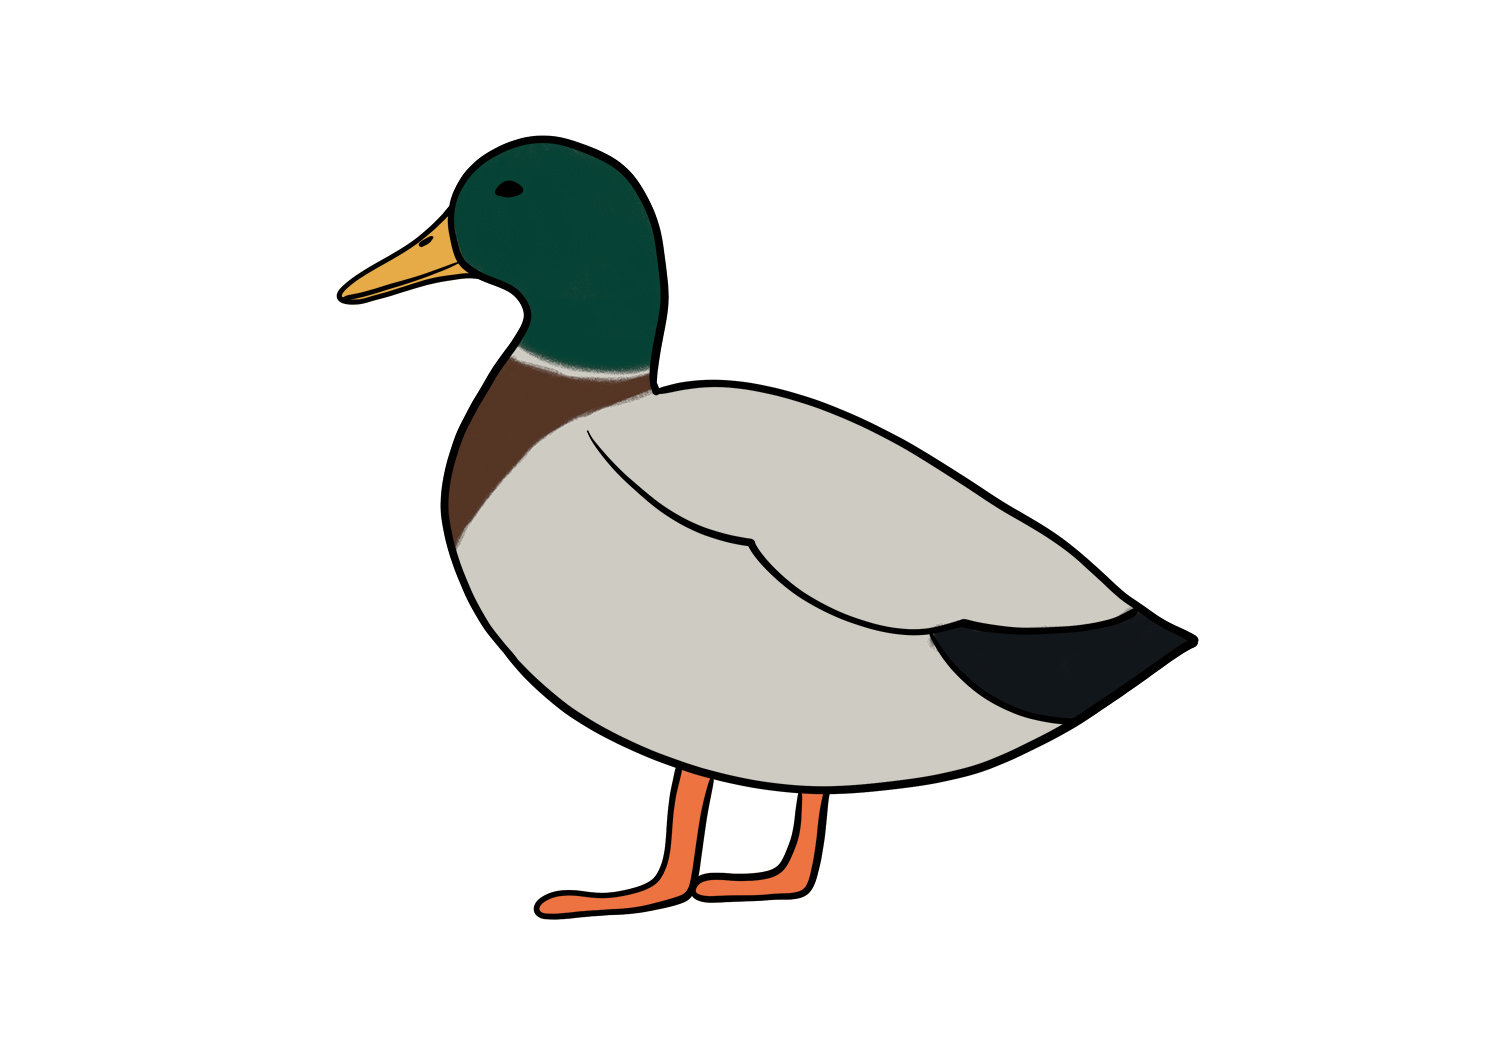
\includegraphics[width=0.5\textwidth]{images/duck.jpg}
    % \end{figure}
    }

    %\includegraphics[width=0.4\textwidth]{duck_joke.png} % Replace with a joke image of a duck
    %\includegraphics[width=0.6\textwidth]{duck_curve.png} % Replace with real duck curve of renewable energy
\end{frame}
\nc{\captionducktwo}{\caption{Comparison of Yearly Solar Power Generation, Energy Demand, and Net Energy Demand in Italy.}}
\begin{frame}{Duck two}
    \only<1>{
\begin{figure}[t!]
    \centering
    \begin{tikzpicture}
        \begin{axis}[
            width=15cm,
            height=7cm,
            xlabel={Month},
            ylabel={ \% of energy demand},
            xtick={0, 63, 120, 180, 240, 310},
            xticklabels={Jan,  Mar,  Jul,  Set, Nov, Dec},
            legend pos=north west,
            legend style={draw=none},
            grid=major
        ]
        
        \addplot+[
            thick,
            mark=none,
            color=green!90
        ] table [
            x index=0,
            y index=1,
            col sep=space
        ] {plots/y3_solar.csv};
       

        \addplot+[
            thick,
            mark=none,
            color=blue!90
        ] table [
            x index=0,
            y index=1,
            col sep=space
        ] {plots/y2_demand.csv};
        

        \addplot+[
            thick,
            mark=none,
            color=red
        ] table [
            x index=0,
            y index=1,
            col sep=space
        ] {plots/y2_net.csv};
        \legend{Solar power, Demand, Net energy}
        \end{axis}
        
        \end{tikzpicture}
        \captionducktwo
\end{figure}
}
\only<2>{
    \begin{figure}[t!]
            \centering
            \begin{tikzpicture}
                %\node  at (axis cs: 3,4) {\duckone};
                \begin{axis}[
                    width=15cm,
                    height=7cm,
                    xlabel={Month},
                    ylabel={ \% of energy demand},
                    xtick={0, 63, 120, 180, 240, 310},
                    xticklabels={Jan,  Mar,  Jul,  Set, Nov, Dec},
                    legend pos=north west,
                    legend style={draw=none},
                    grid=major
                ]
                
                \addplot+[
                    thick,
                    mark=none,
                    color=green!20
                ] table [
                    x index=0,
                    y index=1,
                    col sep=space
                ] {plots/y3_solar.csv};
               
        
                \addplot+[
                    thick,
                    mark=none,
                    color=blue!20
                ] table [
                    x index=0,
                    y index=1,
                    col sep=space
                ] {plots/y2_demand.csv};
                
        
                \addplot+[
                    thick,
                    mark=none,
                    color=red
                ] table [
                    x index=0,
                    y index=1,
                    col sep=space
                ] {plots/y2_net.csv};
                \legend{Solar power, Demand, Unmet Demand};

                \end{axis}
                %\node {\duckone};
        \end{tikzpicture}   
        \begin{tikzpicture}
            \ducktwo
        \end{tikzpicture}
        \captionducktwo
    \end{figure}}
    

%\includegraphics[width=0.4\textwidth]{duck_joke.png} % Replace with a joke image of a duck
%\includegraphics[width=0.6\textwidth]{duck_curve.png} % Replace with real duck curve of renewable energy

\end{frame}
